\documentclass[12pt]{article}

\usepackage{amsmath, color}
\usepackage{mdwmath}
\usepackage{amssymb, epsf, epsfig, textcomp}
\renewcommand{\baselinestretch}{1.3}
\usepackage{a4wide}
\newcommand{\argmin}{\mathop{\mathrm{argmin}}}
\usepackage{caption}
\usepackage{subcaption}
\usepackage{mathtools}
\usepackage{listings}
\lstdefinestyle{myCustomMatlabStyle}{
	basicstyle=\ttfamily\footnotesize,
	breaklines=true,
	language=Matlab,
	numbers=left,
	stepnumber=1,
	numbersep=10pt,
	tabsize=4,
	showspaces=false,
	showstringspaces=false
}
\begin{document}
	\noindent\rule{\textwidth}{2pt}
	\begin{center}
		{\bf Technical University of Crete}\\
		{\bf School of Electrical and Computer Engineering} \\
		Course: {\bf Wireless Communications 2022-2023} \\
		Exercise 2 (120/1000) \\
		Report Delivery Date: 24 November 2022 \\
		Instructor: Athanasios P. Liavas \\
	\end{center}
	{\bf Student: }Alevrakis Dimitrios 2017030001\\
	\rule{\textwidth}{.5pt}
	\vskip .1cm
	\noindent
	
	\begin{enumerate}
		\item[\bf Part 1]
		\begin{enumerate}
			\item[\bf 1]
			The block fading channels are created as described below:
			\begin{lstlisting}[language=octave]
h = zeros(M,N);
for div = 1 : M
	h(div,:) = (randn(1,N) + 1i*randn(1,N))*sqrt(1/2);
end
			\end{lstlisting}
			Where $M$ the desired diversity, meaning the number of receive antennae.
			
			\item[\bf 2]
			The transmitted 4-QAM symbols are created as described below:
			\begin{lstlisting}[language=octave]
s = 1 - (randi(2,[1,N])-1)*2 + 1i*(  1 - (randi(2,[1,N])-1)*2 );
			\end{lstlisting}
		
			\item[\bf 3]
			The White Gaussian noise is created as described below:
			\begin{lstlisting}[language=octave]
n = zeros(M,N);
for div = 1:M
	n(div,:) = ( randn(1,N) + 1i*randn(1,N) )*sqrt(N_0/2);
end
			\end{lstlisting}
			
			Therefore the received signal on each antenna is:
			\begin{lstlisting}[language=octave]
r = zeros(M,N);
for div = 1:M
	r(div,:) = h(div,:).*s + n(div,:);
end
			\end{lstlisting}
		
			The transmitted signal power:
			\begin{align*}
				P_{TX} = \mathcal{E}[s^2] = \frac{1}{N}\sum_{i=1}^{N}|s_i|^2 = \frac{1}{N}\sum_{i=1}^{N}|\pm1 \pm i|^2 = \frac{1}{N}\sum_{i=1}^{N}2 = 2
			\end{align*}
			Therefore the SNR in this case:
			\begin{align*}
				SNR_{db}=10log_{10}\frac{P_{TX}}{P_{noise}}=10log_{10}\frac{2}{N_0}
			\end{align*}
		
			In order to get the desired SNR:
			\begin{align*}
				N_0 = \frac{2}{10^{\frac{SNR_{db}}{10}}}
			\end{align*}
		
			\item[\bf 4]
			Using the Maximum Ratio Combining(MRC) method we define:
			\begin{align*}
				R\coloneqq\frac{{\bf h}^H}{||{\bf h||}}{\bf Y}
			\end{align*}
			and decide using the Maximum Likelihood(ML) method
			\begin{align*}
				{\bf x}^* = \underset{{\bf X}}{min}||{\bf R}-{\bf X}||^2
			\end{align*}
		
			\newpage
			\item[\bf 5]
			\begin{figure}[h!]
				\centering
				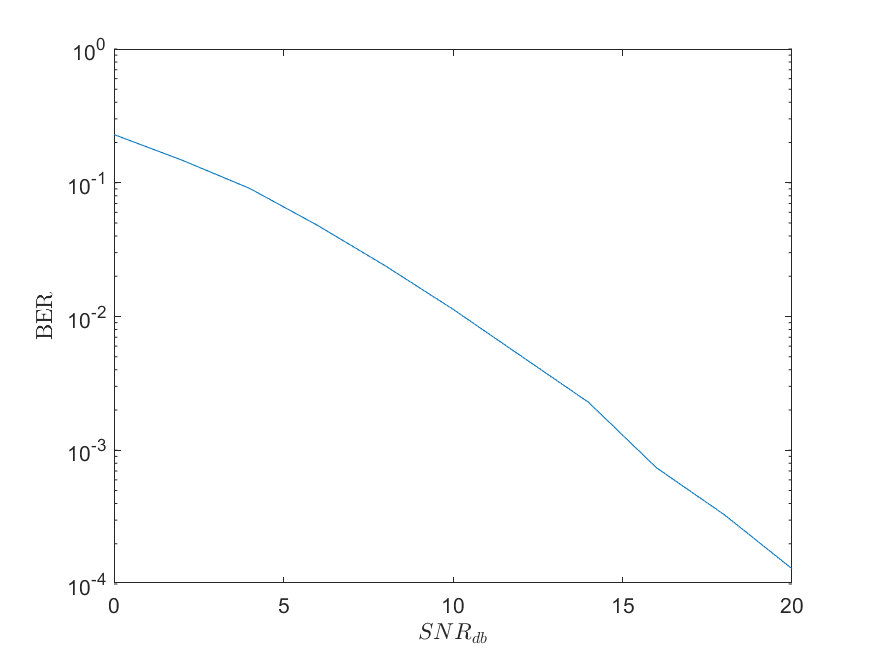
\includegraphics[width=0.5\textwidth]{fig1.png}
				\caption{MRC method: BER for $SNR_{db}=[0:2:20]$}
			\end{figure}
			
			
			\item[\bf 6]
			The theoretical BER:
			\begin{align*}
				BER_{Theoretical}=\begin{pmatrix}
					2M-1 \\ M
				\end{pmatrix}\frac{1}{4^MSNR_{db}^M}
			\end{align*}
			\begin{figure}[h!]
				\centering
				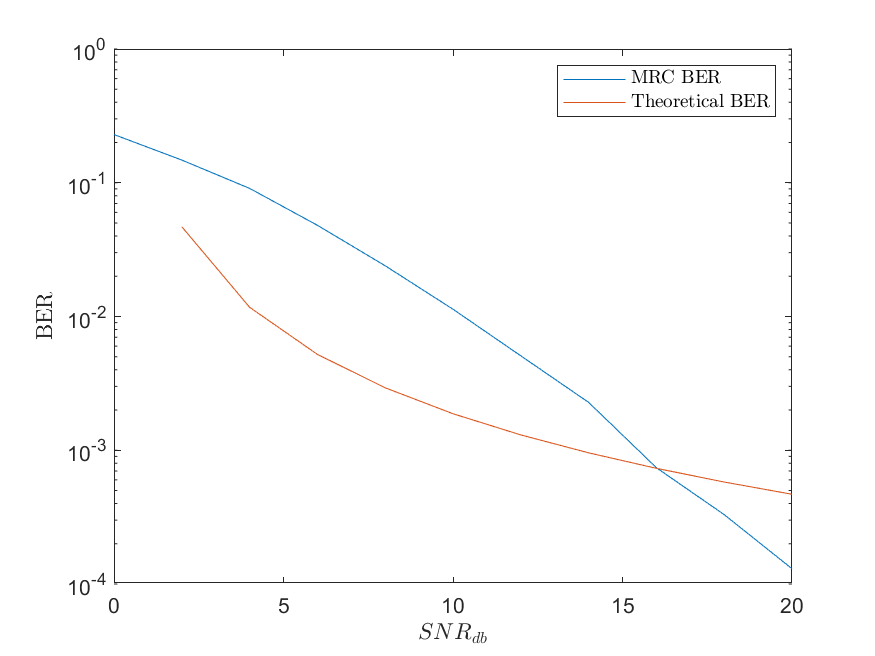
\includegraphics[width=0.5\textwidth]{fig2.png}
				\caption{MRC method: Experimental and Theoretical BER for $SNR_{db}=[0:2:20]$}
			\end{figure}
			
			\item[\bf 7]
			\begin{itemize}
				\item Steps 1-2 are executed the same as before.
				\item In the Transmit Beamforming method the received signal is considered to be:
				\begin{align*}
					Y = ||{\bf h}||X + W
				\end{align*}
			
				\item Using ML we decide the received signal:
				\begin{align*}
					{\bf x}^* = \underset{{\bf X}}{min}||Y-{\bf X}||^2
				\end{align*}
				
				\item 
				\begin{figure}[h!]
					\centering
					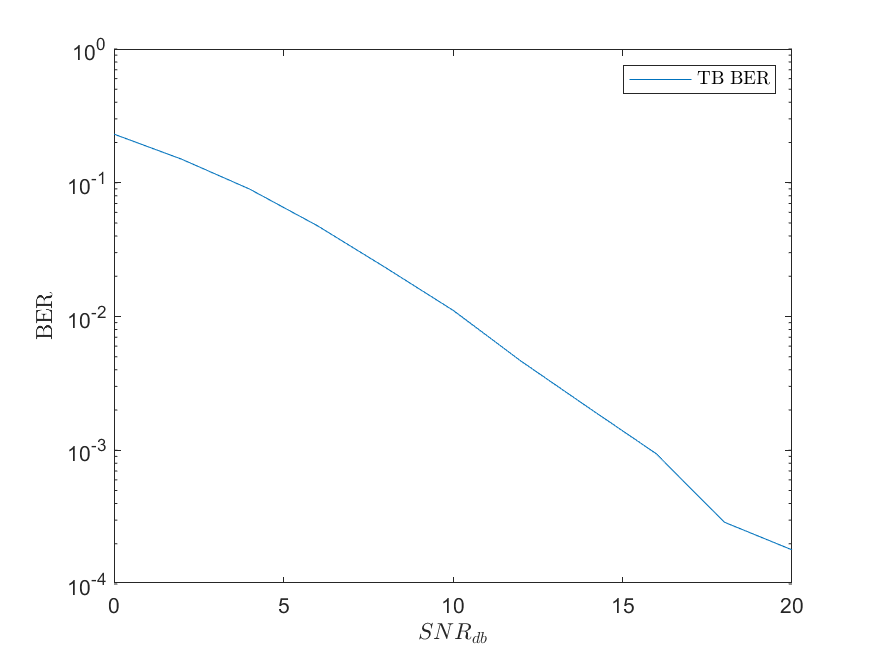
\includegraphics[width=0.5\textwidth]{fig3.png}
					\caption{TB method: BER for $SNR_{db}=[0:2:20]$}
				\end{figure}
			\end{itemize}
			\item[\bf 8]
			\begin{figure}[h!]
				\centering
				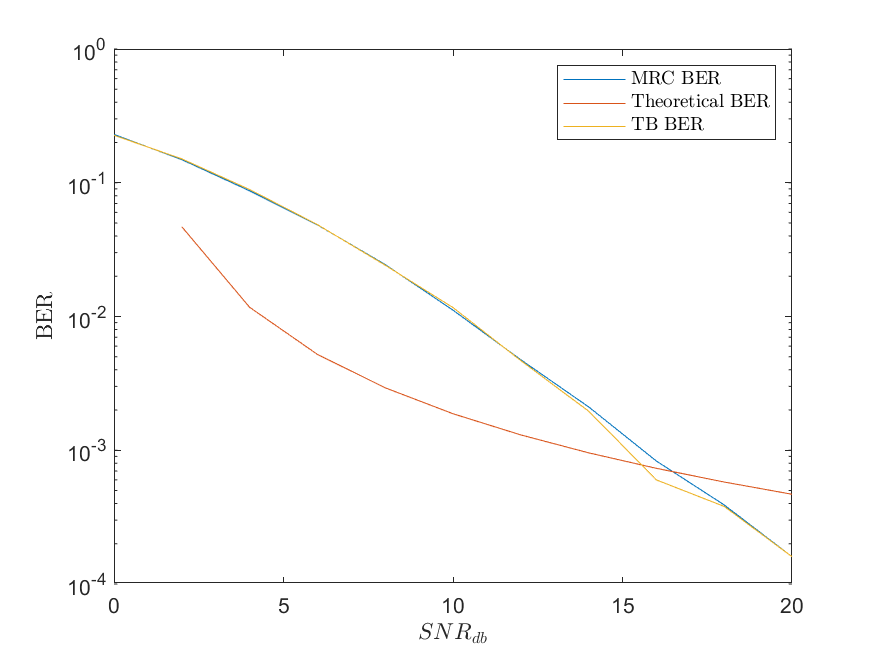
\includegraphics[width=0.5\textwidth]{fig4.png}
				\caption{MRC-TB-Theoretical: BER for $SNR_{db}=[0:2:20]$}
			\end{figure}
		
			\newpage
			\item[\bf 9]
			\item[\bf 10]
			\item[\bf 11]
		\end{enumerate}
		
		\item[\bf Part 2]
		\begin{enumerate}
			\item[\bf 1]
			\item[\bf 2]
			\item[\bf 3]
			\item[\bf 4]
		\end{enumerate}
	\end{enumerate}
	
\end{document}
